\documentclass[12pt,compress,aspectratio=169]{beamer}
\usetheme{metropolis}
\setbeamersize{text margin left=.5cm,text margin right=.5cm}
\usepackage[lf]{carlito}
\usepackage{siunitx}
\usepackage{tikz}
\usepackage{mathpazo}
\usepackage{bm}
\usepackage{mathtools}
\usepackage[ISO]{diffcoeff}
\diffdef{}{ op-symbol=\mathsf{d} }
\usepackage{xcolor,colortbl}

\setmonofont{Ubuntu Mono}
\setlength{\parskip}{0pt}
\renewcommand{\baselinestretch}{1}

\sisetup{
  inter-unit-product=\cdot,
  per-mode=symbol
}

\tikzset{
  >=latex
}

%\newcommand{\iii}{\hat{\bm\imath}}
%\newcommand{\jjj}{\hat{\bm\jmath}}
%\newcommand{\kkk}{\hat{\bm k}}

\usepackage{pgfplots}

\usetikzlibrary{decorations.pathmorphing,patterns}

\title{Classes 9 \& 10: Harmonic Motion}
\subtitle{AP Physics C}
\author[TML]{Dr.\ Timothy Leung}
\institute{Olympiads School}
\date{Updated: Summer 2022}

\newcommand{\pic}[2]{
  \includegraphics[width=#1\textwidth]{#2}
}
\newcommand{\eq}[2]{
  \vspace{#1}{\Large
    \begin{displaymath}
      #2
    \end{displaymath}
  }
}
%\newcommand{\iii}{\ensuremath\hat{\bm{\imath}}}
%\newcommand{\jjj}{\ensuremath\hat{\bm{\jmath}}}
%\newcommand{\kkk}{\ensuremath\hat{\bm{k}}}
\newcommand{\iii}{\ensuremath\hat\imath}
\newcommand{\jjj}{\ensuremath\hat\jmath}
\newcommand{\kkk}{\ensuremath\hat k}



\begin{document}

\begin{frame}
  \maketitle
\end{frame}



\section{Introduction}

\begin{frame}{Oscillatory Systems}
  In Class 3 (Work and Energy), we studied several oscillatory systems using
  the law of conservation of energy. But it is clear that the law of
  conservation of energy does not tell us \emph{why} the masses oscillate.

  \vspace{.1in}
  \begin{columns}[T]
    \column{.32\textwidth}
    \centering

    {\footnotesize Horizontal Spring-Mass System:}

    \vspace{.3in}
    \begin{tikzpicture}[scale=.85]
      \draw[mass] (3,.5) rectangle +(1,1);
      \draw[thick,
        decoration={aspect=.3,segment length=6, amplitude=2.5mm, coil},
        decorate] (0,1)--(3,1);
      \fill[pattern=north east lines] (4.3,0.5)--(4.3,.3)--(-.2,.3)
      --(-.2,2)--(0,2)--(0,.5)--cycle;
      \draw[very thick] (0,2)--(0,.5)--(4.3,.5);
    \end{tikzpicture}

    \vspace{.23in}
    \begin{displaymath}
      K+U_e=\text{constant}
    \end{displaymath}
    
    \column{.32\textwidth}
    \centering

    {\footnotesize Vertical Spring-Mass System:}\\
    \begin{tikzpicture}
      \draw[mass] (.7,1.9) rectangle +(.6,.6);
      \draw[thick,
        decoration={aspect=.3,segment length=6, amplitude=2.5mm, coil},
        decorate] (1,5)--(1,2.5); 
      \fill[pattern=north east lines] (0,5) rectangle (2,5.2);
      \draw[very thick] (0,5)--(2,5);
    \end{tikzpicture}
    \begin{displaymath}
      K+U_e+U_g=\text{constant}
    \end{displaymath}
    
    \column{.32\textwidth}
    \centering

    {\footnotesize Simple Pendulum System:}\\
    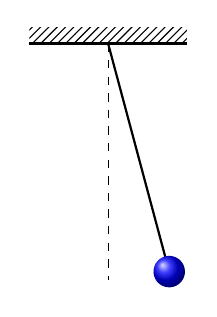
\begin{tikzpicture}
      \fill[pattern=north east lines] (-1,0) rectangle (1,.2);
      \draw[very thick] (-1,0)--(1,0);
      \begin{scope}[rotate=15]
        \draw[thick] (0,0)--(0,-3);% node[midway,right]{$\ell$};
        \shade[ball color=blue] (0,-3) circle (.2);
      \end{scope}
      \draw[dashed,thin] (0,0)--(0,-3);
    \end{tikzpicture}
    \begin{displaymath}
      K+U_g=\text{constant}
    \end{displaymath}
  \end{columns}  
\end{frame}


\begin{frame}{Oscillatory Systems}
  To understand how these systems oscillate, we have to go back to the
  dynamics (i.e.\ using free-body diagrams and second law of motion) of such
  a system. These types of oscillatory motion is called \textbf{harmonic motion}
\end{frame}



%\section{Hooke's Law}
%
%\begin{frame}{Review: Hooke's Law}
%  Hooke's law for an ideal spring relates the \textbf{spring force} $\vec F_s$
%  exerted by a compressed or stretched spring onto another object to the
%  \textbf{spring constant} $k$\footnote{It is the stiffness of the spring, also
%  called \textbf{Hooke's constant}, \textbf{force constant}, or the
%  \textbf{spring rate} of the spring. It depends on both the geometry of the
%  spring, as well as the material properties of the spring}, and the spring's
%  displacement $\vec x$:
%
%  \eq{-.1in}{
%    \boxed{\vec F_s=-k\vec x}
%  }
%  
%  \begin{center}
%    \begin{tabular}{l|c|c}
%      \rowcolor{pink}
%      \textbf{Quantity} & \textbf{Symbol} & \textbf{SI Unit} \\ \hline
%      Spring force        & $\vec F_s$ & \si\newton \\
%      Spring constant     & $k$        & \si{\newton\per\metre}\\
%      Spring Displacement & $\vec x$   & \si\metre
%    \end{tabular}
%  \end{center}
%  \vspace{.3in}
%\end{frame}
%
%
%
%\begin{frame}{Review: Elastic Potential Energy}
%  Applying Hooke's law in the work equation gives the amount of \textbf{elastic
%    potential energy} stored in the spring when it is compressed or stretched:
%
%  \eq{-.1in}{
%    W=\int^{x_1}_{x_0}F_s\dl x=-\int^{x_1}_{x_0}kx\dl x
%    =-\frac12kx^2\Big|^{x_1}_{x_0}=-\Delta U_s
%  }
%
%  where elastic potential energy is defined as
%
%  \eq{-.1in}{
%    \boxed{U_s=\frac12kx^2}
%  }
%\end{frame}



\section{Spring-Mass Systems}

\begin{frame}{Horizontal Spring-Mass System}
  Consider the forces acting on a mass connected horizontally to a spring
  without friction:
  \begin{center}
    \begin{tikzpicture}[scale=1.1]
      \draw[thick,<->] (0,1.7)--+(3.5,0)
      node[midway,fill=black!2] {\scriptsize natural length};
      \draw[mass] (5,.5) rectangle (6,1.5);
      \draw[thick,decorate,
        decoration={aspect=.4,segment length=8,amplitude=8,coil}] (0,1)--(5,1);
      \fill[pattern=north east lines] (6.5,.5)--(6.5,.3)--(-0.2,.3)
      --(-.2,2)--(0,2)--(0,.5)--cycle;
      \draw[thick] (6.5,.5)--(0,.5)--(0,2);
      \draw[axes] (7,1)--(7.8,1) node[right]{$+$};
      \draw[dashed] (3.5,-.5)--(3.5,2.2)
      node[above,text width=1.5cm]
      {equilibrium\\(unstretched)\\$x=0$\par};
      \draw[vectors] (3.5,0)--(5,0) node[midway,below]{$\vec x$};
      \fill[red] (5.5,1) circle (.08);
      \draw[vectors,red] (5.5,1)--(5.5,0) node[below]{$\vec F_g$};
      \draw[vectors,red] (5.5,1)--(5.5,2) node[above]{$\vec F_n$};
      \draw[vectors,red] (5.5,1)--(4.5,1) node[above]{$\vec F_s$};
    \end{tikzpicture}
  \end{center}
  \vspace{-.08in}$\vec F_g$ and $\vec F_n$ cancel out, so net force is due only
  to spring force $\vec F_s=-k\vec x$ along the $x$-axis. This is true both
  when the spring is in compression or extension.\footnote{It should be obvious
  that the spring is in extension in the diagram.} The spring force is a
  ``restoring force'' because it always points towards the equilibrium position.
  \vspace{.1in}
\end{frame}



\begin{frame}{Horizontal Spring-Mass System}
  Applying the second law of motion in the $x$-direction:

  \eq{-.1in}{
    \underbracket[1pt]{F_\text{net}}_{=F_s}=ma
    \quad\longrightarrow\quad
    -kx=m\diff[2]xt
  }

  In calculus, this is a \emph{second-order ordinary differential equation
  with constant coefficients}. In standard form:

  \eq{-.1in}{
    \diff[2]xt + \frac kmx=0
  }
\end{frame}



\begin{frame}{Horizontal Spring-Mass System}

  \eq{0in}{
    \diff[2]xt + \frac kmx=0
  }

  The solution to the equation is a function $x(t)$ where the second time
  derivative $\ddot x$ looks like $x$ but with a negative sign. The only two
  functions that satisfy this requirement are the two sinusoidal functions:
  $\sin(t)$ and $\cos(t)$. We start with this general form:
    
  \eq{-.1in}{
    x(t)=A\cos(\omega_0 t-\theta_0)
  }
  
  \vspace{-.15in}Whether to use the sine or cosine function depends on the
  initial conditions; we generally use the function so that we can set the
  phase constant is $\theta_0=0$. Mathematically, the two functions only differ
  in the phase constant $\theta_0$.
\end{frame}



\begin{frame}{Horizontal Spring-Mass System}

  \eq{0in}{
    \diff[2]xt + \frac kmx=0
  }
  
  Starting with the general form and taking time derivatives to obtain the
  velocity and acceleration of the mass:
 
  \vspace{-.2in}{\large
    \begin{align*}
      x(t)&=A\cos(\omega_0 t-\theta_0)\\
      v(t)&=-A\omega_0\sin(\omega_0 t-\theta_0)\\
      a(t)&=-A\omega_0^2\cos(\omega_0 t-\theta_0)=-\omega_0^2x
    \end{align*}
  }
  
  \vspace{.05in}where $\omega_0$ is the angular frequency, $A$ is the
  amplitude, and $\theta_0$ is the phase constant, based on initial conditions.
  This kind of motion is called a \textbf{simplar harmonic motion}, and a
  system that exhibits harmonic motion is a \textbf{harmonic oscillator}
\end{frame}



\begin{frame}{Horizontal Spring-Mass System: Angular Frequency}
  Substituting expressions of $x(t)$ and $a(t)=\ddot x$ back into the ODE, we
  find that the ODE is satisfied if $\omega_0$ is related to the spring
  constant and mass by:

  \eq{-.1in}{
    \boxed{
      \omega_0=\sqrt{\frac km}
    }  }

  The angular frequency for the simple harmonic oscillator is called the
  \textbf{natural frequency}. The period ($T_0$) and frequency ($f_0$) of the
  simple harmonic oscillator are then given by:

  \eq{-.1in}{
    \boxed{
      f_0=\frac{\omega_0}{2\pi}=\frac1{2\pi}\sqrt{\frac km}
    }
    quad\quad
    \boxed{
      T_0=\frac1{f_0}=2\pi\sqrt{\frac mk}
    }
  }
  
  Angular frequency ($\omega_0$), frequency ($f_0$), and period ($T_0$) do not
  depend on amplitude $A$. In many physics textbooks, the term ``natural
  frequency'' may refer to both $\omega_0$ and $f_0$; the term is often used
  interchangeably.
\end{frame}



\begin{frame}{Relationship to Circular Motion}
  The natural frequency of a simple harmonic oscillator is related to the
  angular frequency of a uniform circular motion.
  \begin{columns}
    \column{.3\textwidth}
    \begin{tikzpicture}[scale=.8,thick]
      \draw[axes] (-3,0)--(3,0) node[right]{$x$};
      \draw[axes] (0,-3)--(0,3) node[above]{$y$};
      \draw circle (2.5);
      \begin{scope}[rotate=38]
        \draw[vectors] (0,0)--(2.45,0) node[midway,above]{$R$};
        \draw[mass] (2.5,0) circle (.1);
      \end{scope}
      \draw[axes] (1,0) arc (0:38:1) node[pos=.55,right]{$\theta$};
      \draw[vectors] (0,0)--({2.5*cos(38)},0) node[midway,below]{$x$};
      \draw[vectors] (0,0)--(0,{2.5*sin(38)}) node[midway,left]{$y$};
      \draw[dashed] ({2.5*cos(38)},0)--({2.5*cos(38)},{2.5*sin(38)})
      --(0,{2.5*sin(38)});
    \end{tikzpicture}

    \column{.65\textwidth}
    \begin{itemize}
    \item An object moving in uniform circular motion with radius $R$
      and angular frequency $\omega$. The angular position $\theta(t)$ of the
      object is:

      \eq{-.15in}{
        \theta(t)=\omega t+\theta_0
      }

    \item\vspace{-.2in}The projection onto the $x$ and $y$ axes are therefore:

      \vspace{-.33in}{\large
        \begin{align*}
          x(t) &= R\cos(\omega t+\theta_0)\\
          y(t) &= R\sin(\omega t+\theta_0)
        \end{align*}
      }

    \item The ``radius'' of the circular motion is the amplitude $A$ of the
      harmonic motion. 
    \end{itemize}
  \end{columns}
%Yes, it most certainly is. In essence, the simple harmonic motion is the
%  projection of a uniform circular motion onto an axis. If angular position is
%  given by $\theta(t)=\omega t+\theta_0$, then
  %  $x(t)=r\cos(\theta)=r\cos(
%  which is the same form as
%  Eq.~\ref{eq:ode1}.
  
\end{frame}


\begin{frame}{Displacement, Velocity and Acceleration}
  \begin{columns}
    \column{.4\textwidth}
    \begin{align*}
      x(t)&=A\cos(\omega_0 t-\phi)\\
      v(t)&=-A\omega_0\sin(\omega_0 t-\phi)\\
      a(t)&=-A\omega_0^2\cos(\omega_0 t-\phi)=-\omega_0^2x
    \end{align*}

    \column{.6\textwidth}
    \begin{tikzpicture}[yscale=.5]
      \draw[axes] (0,-2)--(0,2) node[left]{$x$};
      \draw[axes] (-1,0)--(8,0) node[right]{$t$};
      \draw[functions,smooth,samples=80,domain=0:7.5]
      plot(\x,{1.5*cos(90*\x)});
      
      \draw[axes] (0,-7)--(0,-3)  node[left]{$v$};
      \draw[axes] (-1,-5)--(8,-5) node[right]{$t$};
      \draw[blue,very thick,smooth,samples=80,domain=0:7.5]
      plot(\x,{-1.5*sin(90*\x)-5});
      
      \draw[axes] (0,-12)--(0,-8)  node[left]{$a$};
      \draw[axes] (-1,-10)--(8,-10) node[right]{$t$};
      \draw[violet,very thick,smooth,samples=80,domain=0:7.5]
      plot(\x,{-1.5*cos(90*\x)-10});
    \end{tikzpicture}
  \end{columns}
\end{frame}



\begin{frame}{Cosine vs.\ Sine}
  When would the solution be a cosine, and when would it be a sine?

  \vspace{-.2in}\begin{columns}[T]
    \column{.47\textwidth}
    \begin{center}
      \begin{tikzpicture}[scale=.95]
        \draw[mass] (4,.5) rectangle +(1,1);
        \draw[thick,
          decoration={aspect=.3,segment length=2mm, amplitude=2.5mm, coil},
          decorate] (0,1)--(4,1);
        \fill[pattern=north east lines] (5.5,.5)--(5.5,.3)--(-.2,.3)
        --(-0.2,1.5)--(0,1.5)--(0,.5)--cycle;
        \draw[very thick] (0,1.5)--(0,.5)--(5.5,.5);
        \draw[vectors] (2.5,1.65)--(4,1.65) node[midway,above]{\scriptsize$x(0)=+A$};
        \draw[dashed,thick] (2.5,.2)--(2.5,2)
        node[above=0]{\scriptsize equilibrium};
      \end{tikzpicture}
    \end{center}
    \vspace{-.1in}
    \textbf{Cosine:} The spring is initially stretched to $x(0)=+A$, and the
    mass is released from rest at $t=0$ (i.e.\ $v(0)=0$).
    \vspace{-.1in}
    \begin{align*}
      x(t)&=A\cos(\omega t)\\
      v(t)&=-A\omega\sin(\omega t)\\
      a(t)&=-A\omega^2\cos (\omega t)
    \end{align*}    
    \column{.47\textwidth}
    \begin{center}
      \begin{tikzpicture}[scale=.95]
        \draw[mass] (2.5,.5) rectangle +(1,1);
        \draw[thick,
          decoration={aspect=.3,segment length=1.3mm, amplitude=2.5mm, coil},
          decorate] (0,1)--(2.5,1);
        \fill[pattern=north east lines] (5.5,.5)--(5.5,.3)--(-.2,.3)
        --(-0.2,1.5)--(0,1.5)--(0,.5)--cycle;
        \draw[very thick] (0,1.5)--(0,.5)--(5.5,.5);
        \draw[vectors] (3,1)--+(1,0) node[right]{\scriptsize$v(0)=v_\text{max}$};
        \draw[dashed,thick] (2.5,.2)--+(0,1.8)
        node[above=0]{\scriptsize equilibrium};
      \end{tikzpicture}
    \end{center}
    \vspace{-.1in}
    \textbf{Sine:} If the mass is given a ``tap'' in the ($+$) direction at
    $t=0$ to give it an initial velocity of $v(0)=v_\text{max}$.
    %If the mass is tapped in the ($-$) direction, use $-\sin$.
    \vspace{-.1in}
    \begin{align*}
      x(t)&=A\sin(\omega t)\\
      v(t)&=A\omega\cos(\omega t)\\
      a(t)&=-A\omega^2\sin(\omega t)
    \end{align*}
  \end{columns}
\end{frame}


\begin{frame}{Maximum Speed}
  The maximum speed (i.e.\ magnitude of velocity) of the mass is the
  ``amplitude'' of the velocity function:

  \eq{-.1in}{
    v(t) =-\underbracket[1pt]{A\omega}_{v_\text{max}}\sin(\omega t)
  }

  \vspace{-.05in}Substituting the expression for $\omega=\sqrt{k/m}$, we get
  
  \eq{-.1in}{
    v_\text{max}=A\omega=A\sqrt{\frac km}
  }

  We can also obtain this result by solving the law of conservation of energy
  problem. 
\end{frame}



\begin{frame}{Maximum Acceleration}
  Likewise, the maximum magnitude of acceleration of the mass is the
  ``amplitude'' of the acceleration function:

  \eq{-.1in}{
    a(t)=-\underbracket[1pt]{A\omega^2}_{a_\text{max}}\cos(\omega t)
  }

  \vspace{-.05in}Again, substituting the expression for $\omega=\sqrt{k/m}$, we
  get:
  
  \eq{-.1in}{
    a_\text{max}=A\omega^2=A\frac km
  }

  We can also obtain this result using the original differential equation.
\end{frame}



\begin{frame}{Side Note \#1}
  \textbf{Side Note \#1:} For anyone with more experiences with calculus,
  you will know that the solution to any ODE is the linear combination of
  \emph{all} possible solutions\footnote{From an even broader discussions on
  mathematics, all the possible solutions to the ODE must be functions that are
  \emph{orthogonal} to each other.}, i.e.:

  \eq{-.1in}{
    x(t)=c_1\sin(\omega_0 t)+c_2\cos(\omega_0 t)
  }

  \vspace{-.1in}Where $c_1$ and $c_2$ are coefficients based on initial
  position $x_0$ and velocity $v_0$.\footnote{Trigonometric identities can be
  used to show that the solution form shown in previous slides is identical.}
\end{frame}



\begin{frame}{Side Note \#2}
  \textbf{Side Note \#2:} Another function that we can be try is the
  exponential function, where its derivatives is related to the function
  itself. However, the second derivative of $e^{\omega_0t}$ does not have the
  negative sign that is needed to solve the problem.

  \eq{-.1in}{
    x(t)=e^{\omega_0t}\quad\rightarrow\quad
    \diff[2]xt=\omega_0^2 e^{\omega_0t}=\omega_0^2x
  }

  But if the exponential function is \emph{imaginary}:

  \eq{-.1in}{
    x(t)=e^{i\omega_0t}
  }

  \vspace{-.1in}Then\ldots
\end{frame}



\begin{frame}{Side Note \#2}
  The second derivative \emph{does} in fact have the negative sign:

  \vspace{-.3in}{\large
    \begin{align*}
      x&=e^{i\omega_0t}\\
      \dot x&=i\omega_0e^{i\omega_0t}\\
      \ddot x&=i^2\omega_0^2 e^{i\omega_0t}=-\omega_0^2 e^{i\omega_0t}
    \end{align*}
  }
  
  This should not come as a surprise, since the complex exponential function
  and the sinusoidal functions are related:

  \eq{-.1in}{
    e^{i\omega_0t}=\cos(\omega_0t)+i\sin(\omega_0t)
  }
\end{frame}



\begin{frame}{Vertical Spring-Mass System}
  \begin{columns}
    \column{.3\textwidth}
    \begin{tikzpicture}[scale=1.3]
      \draw[mass] (.7,1.7) rectangle (1.3,2.3);
      \draw[thick,
        decoration={aspect=0.3,segment length=2mm, amplitude=2.5mm, coil},
        decorate] (1,5)--(1,2.5); 
      \fill[pattern=north east lines] (0,5) rectangle (2,5.2);
      \draw[very thick] (0,5)--(2,5);
      \draw[vectors,red] (1,2)--(1,1.2) node[right]{$\vec F_g$};
      \draw[vectors,red] (1,2)--(1,2.8) node[right]{$\vec F_s$};
      \fill[red] (1,2) circle (.05);
      \draw[axes] (1,1)--(1,.5) node[below]{$+$};
      \draw[vectors] (.3,4)--(.3,2.3) node[midway,left]{$x$};
      \draw[vectors] (1.7,4)--(1.7,3.5) node[midway,right]{$B$};
      \begin{scope}[thick,dashed]
        \draw (0,4)--(2,4) node[right]{\scriptsize unstretched};
        \draw (0,3.5)--(2,3.5) node[right]{\scriptsize equilibrium};
      \end{scope}
    \end{tikzpicture}

    \column{.7\textwidth}
    For a vertical spring-mass system, we must consider
    {\color{purple}weight $F_g=mg$} as well:

    \eq{-.1in}{
      {\color{purple}F_g}-kx=m\diff[2]xt
    }

    But since $F_g$ is a constant force, the only change in the solution is the
    addition of a constant $B$ in the expression of $x(t)$:
    
    \vspace{-.3in}{\large
      \begin{align*}
        x(t) &= A\cos(\omega_0 t-\theta_0) +B\\
        v(t) &= -A\omega_0\sin(\omega_0 t-\theta_0)\\
        a(t) &= -A\omega_0^2\cos(\omega_0 t-\theta_0)
      \end{align*}
    }
  \end{columns}
\end{frame}



\begin{frame}{Vertical Spring-Mass System}
  \begin{columns}
    \column{.3\textwidth}
    \begin{tikzpicture}[scale=1.3]
      \draw[mass] (.7,1.7) rectangle (1.3,2.3);
      \draw[thick,
        decoration={aspect=0.3,segment length=2mm, amplitude=2.5mm, coil},
        decorate] (1,5)--(1,2.5); 
      \fill[pattern=north east lines] (0,5) rectangle (2,5.2);
      \draw[very thick] (0,5)--(2,5);
      \draw[vectors,red] (1,2)--(1,1.2) node[right]{$\vec F_g$};
      \draw[vectors,red] (1,2)--(1,2.8) node[right]{$\vec F_s$};
      \fill[red] (1,2) circle (.05);
      \draw[axes] (1,1)--(1,.5) node[below]{$+$};
      \draw[vectors] (.3,4)--(.3,2.3) node[midway,left]{$x$};
      \draw[vectors] (1.7,4)--(1.7,3.5) node[midway,right]{$B$};
      \begin{scope}[thick,dashed]
        \draw (0,4)--(2,4) node[right]{\scriptsize unstretched};
        \draw (0,3.5)--(2,3.5) node[right]{\scriptsize equilibrium};
      \end{scope}
    \end{tikzpicture}

    \column{.7\textwidth}
    $B$ is found by substituting $x$ and $\ddot x$ into the ODE. It is the
    stretch of the spring due to its own weight:
    
    \eq{-.1in}{
      B=\frac{mg}k
    }

    Angular frequency (natural frequency) remains the same as the horizontal
    case:

    \eq{-.1in}{
      \omega_0=\sqrt{\frac km}
    }
  \end{columns}
\end{frame}



\begin{frame}{Conservation of Energy in a Spring-Mass System}

  In the spring-mass systems, if there are no frictional losses\footnote{i.e.\
  from kinetic friction, drag and other damping forces}, then the only
  forces doing work are the spring force (horizontal and vertical) and gravity
  (vertical). Both forces are \emph{conservative}, therefore the total
  mechanical energy is conserved:

  \eq{-.1in}{
    K + U_s + U_g = K' + U_s' + U_g'
  }
  
  For the horizontal spring-mass system, the total energy of the simple harmonic
  oscillator is:
    
  \eq{-.1in}{
    \boxed{E_T=\frac12kA^2}
  }
  
  \vspace{.2in}
\end{frame}



\begin{frame}{Simple Example}
  \textbf{Example:} A mass suspended from a spring is oscillating up and
  down. Consider the following two statements:
  \begin{enumerate}
  \item At some point during the oscillation, the mass has zero velocity but it
    is accelerating
  \item At some point during the oscillation, the mass has zero velocity and
    non-zero acceleration.
  \end{enumerate}

  \begin{enumerate}[(A)]
  \item Both occur at some time during the oscillation
  \item Neither occurs during the oscillation
  \item Only (1) occurs
  \item Only (2) occurs
  \end{enumerate}
\end{frame}



\begin{frame}{Another Example}
  \textbf{Example:} An object of mass \SI5{\kilo\gram} hangs from a spring
  and oscillates with a period of \SI{.5}\second. By how much will the
  equilibrium length of the spring be shortened when the object is removed.
  \begin{enumerate}[(A)]
  \item\SI{.75}{\centi\metre}
  \item\SI{1.5}{\centi\metre}
  \item\SI{3.1}{\centi\metre}
  \item\SI{6.2}{\centi\metre}
  \end{enumerate}
\end{frame}



\section{Simple Pendulum}

\begin{frame}{What About a Simple Pendulum?}
  \begin{columns}
    \column{.75\textwidth}
    \begin{itemize}
    \item Pendulums also exhibit oscillatory motion
    \item In a \textbf{simple pendulum}, all of the mass is concentrated at the
      end point 
    \item Two forces act on the mass: weight $\vec F_g$ and tension $\vec F_T$
    \item It has been shown in Class 6 (circular motion) that when the mass is
      deflected by an angle $\theta$, the tangential force is
      $F_\text{tangent}=-mg\sin\theta$
    \item No need to worry about the radial direction; it does not contribute
      to the restoring force
    \end{itemize}

    \column{.25\textwidth}
    \centering 
    \begin{tikzpicture}
      \fill[pattern=north east lines] (-1,0) rectangle (1,0.2);
      \draw[thick] (-1,0)--(1,0);
      \begin{scope}[rotate=20]
        \draw[thick] (0,0)--(0,-5) node[midway,right]{$\ell$};
        \shade[ball color=blue] (0,-5) circle (.2) node[below right]{$m$};
        \draw[vectors,red,dotted] (0,-5)--(-1.5*sin{20},-5)
        node[left,fill=yellow!10]{$mg\sin\theta$};
        \draw[vectors,red] (0,-5)--(0,-3) node[left]{$\vec F_T$};
        \draw[vectors,red,rotate around={-20:(0,-5)}] (0,-5)--(0,-6.5)
        node[below]{$\vec F_g$};
      \end{scope}
      \draw[axes] (0,-2) arc (270:290:2) node[midway,below]{$\theta$};
      \draw[dashed] (0,0)--(0,-5);
      \draw[dashed] (0,-5) arc (270:295:5);
      \draw[dashed] (0,-5) arc (270:255:5);
    \end{tikzpicture}
  \end{columns}
\end{frame}



\begin{frame}{The Simple Pendulum}
  \begin{columns}
    \column{.77\textwidth}
    Substitute $F_\text{tangent}$ into the second law of motion, and cancelling
    $m$:

    \eq{-.2in}{
      F_\text{tangent}=ma_\text{tangent}\quad\rightarrow\quad
      -mg\sin\theta=m\ell\diff[2]{\theta}t
    }

    \vspace{-.15in}Solving this ODE is difficult because of the $\sin\theta$
    term. However, we can simplify the problem by using the Taylor series
    expansion of the sine function:

    \eq{-.1in}{
      \sin\theta
      =\theta-\frac{\theta^3}{3!}+\frac{\theta^5}{5!}-\frac{\theta^7}{7!}+\cdots
    }
    
    which shows that for small angles, $\sin\theta\approx\theta$
    
    \column{.22\textwidth}
    \centering
    \begin{tikzpicture}
      \fill[pattern=north east lines] (-1,0) rectangle (1,0.2);
      \draw[thick] (-1,0)--(1,0);
      \begin{scope}[rotate=20]
        \draw[thick] (0,0)--(0,-5) node[midway,right]{$\ell$};
        \shade[ball color=blue] (0,-5) circle (.2) node[below right]{$m$};
      \end{scope}
      \draw[axes] (0,-2) arc (270:290:2) node[midway,below]{$\theta$};
      \draw[dashed] (0,0)--(0,-5);
      \draw[dashed] (0,-5) arc (270:295:5);
      \draw[dashed] (0,-5) arc (270:255:5);
    \end{tikzpicture}
  \end{columns}
\end{frame}



\begin{frame}{The Simple Pendulum}
  \begin{columns}
    \column{.77\textwidth}
    For small angles of $\theta$, the ODE reduces to the same form as the
    spring-mass system

    \eq{-.1in}{
      \diff[2]{\theta}t + \frac g\ell\theta=0
    }

    So how small is ``small angle''? That depends on what tolerance (the
    number of significant figures) is needed in the answer.
    
    \column{.22\textwidth}
    \begin{tikzpicture}
      \fill[pattern=north east lines] (-1,0) rectangle (1,0.2);
      \draw[thick] (-1,0)--(1,0);
      \begin{scope}[rotate=20]
        \draw[thick] (0,0)--(0,-5) node[midway,right]{$\ell$};
        \shade[ball color=blue] (0,-5) circle (.2) node[below right]{$m$};
      \end{scope}
      \draw[axes] (0,-2) arc (270:290:2) node[midway,below]{$\theta$};
      \draw[dashed] (0,0)--(0,-5);
      \draw[dashed] (0,-5) arc (270:295:5);
      \draw[dashed] (0,-5) arc (270:255:5);
    \end{tikzpicture}
  \end{columns}
\end{frame}



\begin{frame}{Solutions to the ODE for the Simple Pendulum}
  The solution for $\theta(t)$ is a sinusoidal function, like the spring-mass
  system:

  \eq{-.1in}{
    \boxed{\theta(t)=\theta_\text{max}\cos(\omega_0 t-\phi)}
  }

  where $\theta_\text{max}$ is the maximum deflection (amplitude), and $\phi$
  is a phase shift based on the initial condition of the pendulum. (If the
  oscillation begins at amplitude, then $\phi=0$) The natural frequency of
  the oscillation ($\omega_0$ and $f_0$) and period ($T_0$) are given by:
    
  \eq{-.1in}{
    \boxed{
      \omega_0=\sqrt{\frac g\ell}      
    }
    \quad\rightarrow\quad
    \boxed{
      f_0=\frac{\omega_0}{2\pi}=\frac1{2\pi}\sqrt{\frac g\ell}
    }
    \quad\quad
    \boxed{
      T=\frac1{f_0}=2\pi\sqrt{\frac\ell g}
    }
  }
\end{frame}



\begin{frame}{Solutions to the ODE for the Simple Pendulum}

  %\eq{0in}{
  %  \boxed{\theta(t)=\theta_\text{max}\cos(\omega_0 t-\phi)}
  %}

  Again, whether the solution for $\theta(t)$ should be a cosine or a sine
  function depends on the initial condition. We want to express the motion
  without worrying about the phase constant.

  \vspace{.1in}
  \begin{columns}
    \column{.5\textwidth}
    \centering
    \begin{tikzpicture}
      \fill[pattern=north east lines] (-2,0) rectangle (2,.2);
      \draw[thick] (-2,0)--(2,0);
      \begin{scope}[rotate=25]
        \draw[thick] (0,0)--(0,-3.5);% node[midway,right]{$\ell$};
        \shade[ball color=blue] (0,-3.5) circle (.2)
        node[below right]{$m$} node[above right]{$v(0)=0$};
      \end{scope}
      \draw[axes] (0,-1.5) arc (270:295:1.5)
      node[pos=0,left]{$\theta(0)=\theta_\text{max}$};
      \draw[dashed] (0,0)--(0,-4);
      \draw[dashed] (0,-3.5) arc (270:300:3.5);
      \draw[dashed] (0,-3.5) arc (270:240:3.5);
    \end{tikzpicture}

    \eq{-.3in}{
      \theta(t)=\theta_\text{max}\cos(\omega_0 t)
    }

    \column{.5\textwidth}
        \centering
    \begin{tikzpicture}
      \fill[pattern=north east lines] (-2,0) rectangle (2,.2);
      \draw[thick] (-2,0)--(2,0);

      \draw[thick] (0,0)--(0,-3.5);% node[midway,right]{$\ell$};
      \shade[ball color=blue] (0,-3.5) circle (.2) node[below right]{$m$};
      \draw[vectors] (0,-3.5)--+(1.3,0) node[right]{$v(0)=v_\text{max}$};

      \draw[dashed] (0,0)--(0,-4) node[pos=.35,left]{$\theta(0)=0$};
      \draw[dashed] (0,-3.5) arc (270:300:3.5);
      \draw[dashed] (0,-3.5) arc (270:240:3.5);
    \end{tikzpicture}

    \eq{-.3in}{
      \theta(t)=\theta_\text{max}\sin(\omega_0 t)
    }

  \end{columns}
\end{frame}


\begin{frame}{Velocity and Acceleration}

  Given the position of the pendulum as a function of time:
  
  \eq{-.1in}{
    \boxed{\theta(t)=\theta_\text{max}\cos(\omega_0 t)}
  }

  The time derivative of $\theta(t)$ gives us its angular
  velocity and velocity about the pivot:

  \eq{-.2in}{
    \boxed{\diff{\theta}t=-\theta_\text{max}\omega_0\sin(\omega_0 t)}
    \;\;\rightarrow\;\;
    \boxed{
      v(t)=\ell\diff{\theta}t=-\ell\theta_\text{max}\omega_0\sin(\omega_0 t)
    }
  }

  The second derivative gives us the angular and tangential accelerations:

  \eq{-.2in}{
    \boxed{\diff[2]{\theta}t=-\theta_\text{max}\omega_0^2\cos(\omega_0 t)}
    \;\;\rightarrow\;\;
    \boxed{
      a_t(t)=\ell\diff[2]{\theta}t=-\ell\theta_\text{max}\omega_0^2\cos(\omega_0 t)
    }
  }

  \textbf{What does $\omega_0$ mean for the simple pendulum case?}
\end{frame}




\begin{frame}{The meaning of $\omega_0$}

  \begin{columns}
    \column{.27\textwidth}
    \centering
    \begin{tikzpicture}[scale=.9]
      \fill[pattern=north east lines] (-2,0) rectangle (2,.2);
      \draw[thick] (-2,0)--(2,0);
      \begin{scope}[rotate=25]
        \draw[thick] (0,0)--(0,-3.5) node[midway,right]{$\ell$};
        \shade[ball color=blue] (0,-3.5) circle (.2)
        node[below right]{$m$};
      \end{scope}

      \begin{scope}[rotate=10]
        \draw[thick,gray] (0,0)--(0,-3.3);
        \shade[ball color=blue,opacity=.3] (0,-3.5) circle (.2);
      \end{scope}

      \begin{scope}[rotate=-20]
        \draw[thick,gray] (0,0)--(0,-3.3);
        \shade[ball color=blue,opacity=.3] (0,-3.5) circle (.2);
      \end{scope}
      
      \draw[axes] (0,-1.5) arc (270:295:1.5) node[right]{$\theta_\text{max}$};
      \draw[dashed] (0,0)--(0,-4);
      \draw[dashed] (0,-3.5) arc (270:300:3.5);
      \draw[dashed] (0,-3.5) arc (270:240:3.5);

      \draw[axes] (-2,-6)--+(4,0) node[right]{$x$};
      \draw[axes] (0,-8)--+(0,4) node[right]{$y$};
      \draw (0,-6) circle (1.48);

      \fill (1.48,-6) circle (.08);
      \draw[red,vectors,rotate around={35:(0,-6)}] (1.48,-6) arc (0:70:1.48)
      node[pos=.2,right]{$\omega_0$};
      
      \draw[dashed] (1.46,-6)--+(0,2.7);
       
      \fill[gray] (.61,-6) circle (.08);
      \fill[gray!70] (.61,-4.66) circle (.08);
      \draw[dashed] (.61,-6)--+(0,2.5);

      \fill[gray] (-1.2,-6) circle (.08);
      \fill[gray!70] (-1.2,-5.13) circle (.08);
      \draw[dashed] (-1.2,-6)--+(0,2.5);
      
      \draw[thick,|<->|] (-1.48,-6.4)--(1.47,-6.4)
      node[midway,below, text width=60]{
        \scriptsize Harmonic motion along the $x$-axis\par
      };
    \end{tikzpicture}
  
    \column{.73\textwidth}
    The meaning of $\omega_0$ for the pendulum is a bit more abstract than in
    the spring-mass case.
    \begin{itemize}
    \item Since we are using a small-angle approximation, we can ``project'' the
      pendulum's location onto the $x$-axis:

      \vspace{-.3in}{\large
        \begin{align*}
          x(t) &=\ell\sin\left(\theta(t)\right)\approx\ell\theta(t)\\
          &=\ell\theta_\text{max}\cos(\omega_0 t)
        \end{align*}
      }

      \vspace{-.05in}$x(t)$ is the pendulum's \textbf{lateral displacement},
      and it is also a simple harmonic motion
      
    \item Now we can relate the oscillation on the $x$ axis to a uniform
      circular motion on the $xy$-plane. $\omega_0$ is the angular frequency
      of this circular motion.
    \end{itemize}
  \end{columns}
\end{frame}



\begin{frame}{How Good is the Small Angle Approximation?}
  \begin{center}
    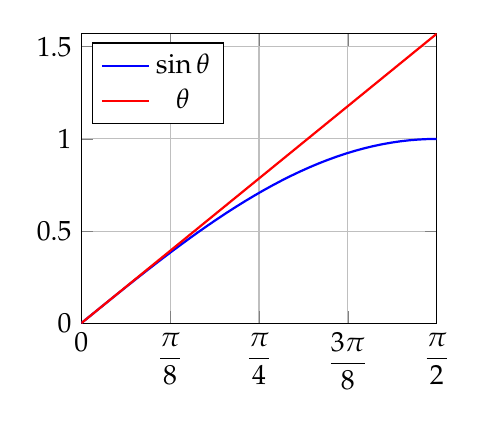
\begin{tikzpicture}
      \begin{axis}[
          width=2.4in,
          xmin=0,xmax=pi/2,
          ymin=0,ymax=pi/2,
          %xlabel=$\theta$ (radian),
          xtick={0,pi/8,pi/4,3*pi/8,pi/2},
          xticklabels={
            0,$\dfrac\pi8$,$\dfrac\pi4$,$\dfrac{3\pi}8$,$\dfrac\pi2$
          },
          grid = both,
          legend pos=north west,
        ]
        \addplot[
          color=blue,
          domain=0:pi/2,
          samples=40,
          style={thick}]{sin(x*180/pi)};
        \addlegendentry{$\sin\theta$}
        \addplot[
          color=red,
          domain=0:pi/2,
          samples=40,
          thick]{x};
        \addlegendentry{$\theta$}
      \end{axis}
    \end{tikzpicture}
    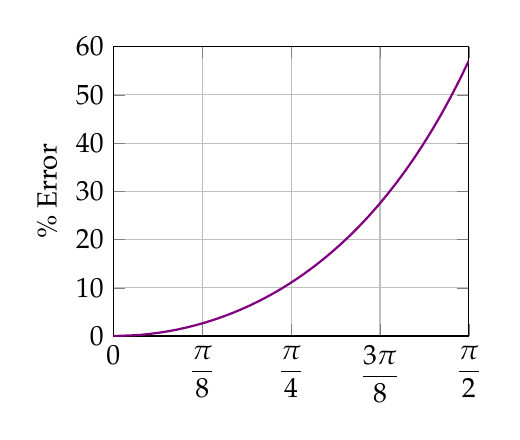
\begin{tikzpicture}
      \begin{axis}[
          width=2.4in,
          ylabel=\% Error,
          xmin=0,xmax=pi/2,
          ymin=0,ymax=60,
          %xlabel=$\theta$ (radian),
          xtick={0,pi/8,pi/4,3*pi/8,pi/2},
          xticklabels={
            0,$\dfrac\pi8$,$\dfrac\pi4$,$\dfrac{3\pi}8$,$\dfrac\pi2$
          },
          ytick={0,10,...,60},
          legend pos=north west,
          grid = both,
        ]
        \addplot[
          color=violet,
          domain=0:pi/2,
          samples=40,
          style=thick
        ]{abs(sin(x*180/pi)-x)/sin(x*180/pi)*100};
      \end{axis}
    \end{tikzpicture}
  \end{center}
  What the maximum angle of deflection can be used depends on the precision
  that the answer requires. Note that the small-angle approximation always
  over-estimates the restoring force, therefore our (approximated) solution
  always under-estimates the period.
\end{frame}



\begin{frame}{Pendulum Example Problem}
  \textbf{Example:} A simple pendulum consists of a mass $m$ attached to a
  light string of length $\ell$. If the system is oscillating through small
  angles, which of the following is true
  \begin{enumerate}[(A)]
  \item The frequency is independent of the acceleration due to gravity, $g$.
  \item The period depends on the amplitude of the oscillation.
  \item The period is independent of the mass $m$.
  \item The period is independent of the length $\ell$.
  \end{enumerate}
\end{frame}



\begin{frame}{A Pendulum Example}
  \textbf{Example:} A bucket full of water is attached to a rope and allowed
  to swing back and forth as a pendulum from a fixed support. The bucket has a
  hole in its bottom that allows water to leak out. How does the period of
  motion change of the bucket with the loss of water?
  \begin{enumerate}[(A)]
  \item The period does not change.
  \item The period continuously decreases.
  \item The period continuously increases.
  \item The period increases to some maximum and then decreases again.
  \end{enumerate}
\end{frame}



\begin{frame}{Think About $g$}
  \textbf{Example:} A little girl is playing with a toy pendulum while riding
  in an elevator. Being an astute and educated observer, she notes that the 
  period of the pendulum is $T=\SI{.5}\second$. Suddenly the cables
  supporting the elevator break and all  of the brakes and safety features fail
  simultaneously. The elevator plunges into free fall. The young girl is
  astonished to discover that the pendulum has:
  \begin{enumerate}[(A)]
  \item continued oscillating with a period of \SI{.5}\second.
  \item stopped oscillating entirely.
  \item decreased its rate of oscillation to have a longer period.
  \item increased its rate of oscillation to have a lesser period.
  \end{enumerate}
\end{frame}



\section{Damped Oscillation}

\begin{frame}{It's Never Perfect}
  In reality, there are friction, or drag, or other damping forces present in
  the spring-mass system, represented schematically by the shock absorber:
  \begin{center}
    \begin{tikzpicture}
      \draw[gray,mass] (3,.5) rectangle (4,1.5);
      \draw[thick,draw=gray,decorate,
        decoration={aspect=.4,segment length=5,amplitude=8,coil}] (0,1)--(3,1);
      \fill[gray,pattern=north east lines] (-.2,2)--(-.2,.3)--(6.7,.3)--(6.7,2)
      --(6.5,2)--(6.5,.5)--(0,.5)--(0,2)--cycle;
      \draw[gray,thick] (0,2)--(0,.5)--(6.5,.5)--(6.5,2);
      \draw[axes] (7.25,1)--(8,1) node[right]{$x$};
      \fill[blue!20!white] (5,.8) rectangle (6,1.2);
      \draw[very thick] (4,1)--(5,1);
      \draw[very thick] (5,.8)--(5,1.2);
      \draw[very thick] (4.9,1.2)--(6,1.2)--(6,.8)--(4.9,.8);
      \draw[very thick] (6,1)--(6.5,1);

      \draw[vectors,pink] (3.5,1)--(3.5,0) node[right]{$\vec F_g$};
      \draw[vectors,pink] (3.5,1)--(3.5,2) node[right]{$\vec F_n$};
      \draw[vectors,pink] (3.5,1)--(2.5,1) node[above]{$\vec F_s$};
      \draw[vectors,red] (3.5,1)--(4.5,1) node[above]{$\vec F_D$};
      \fill[red] (3.5,1) circle (.075);
    \end{tikzpicture}
  \end{center}
  The combined friction, drag, and damping forces are grouped into a single
  damping force ``$\vec F_D$''.
  
  %\uncover<3->{
  %  \vspace{-.1in}The damping force is typically related to velocity, in the
  %  opposite direction:
  %
  %  \eq{-.135in}{
  %    F_D=-bv^n
  %  }
  %
  %  \vspace{-.12in}where $b$ is a positive constant called the \textbf{damping
  %    factor}.
    %The simplest case is to use $n=1$ to represent combined viscous
    %effects. %(Kinetic friction, $n=0$; aerodynamic drag, $n=2$)
  %}
\end{frame}



\begin{frame}{Damped Oscillators}
  In general, the damping force is a function of velocity, and acts in the
  opposite direction to the motion of the mass:
  
  \eq{-.22in}{
    F_D=-bv^n
  }

  \vspace{-.15in}The positive constant $b$ is called the \textbf{damping
    factor}.
  \begin{itemize}
  \item For kinetic friction, $n=0$
  \item For aerodynamic drag, $n=2$, and
  \item For viscous damping, $n\approx 1$
  \end{itemize}
  Usually there is a combination of these forces, so we use $n=1$ to
  approximate the \emph{average}\footnote{Whether this is
  \emph{accurate} will depend on the specific problem that needs to be solved.}.
  %Applying the 2nd law of motion, the differential equation is more complicated:
  %
  %\eq{-.2in}{
  %  -kx-bv=ma
  %}
\end{frame}




\begin{frame}{Damped Oscillator}
  The 2nd-order ODE is obtained by applying second law of motion, this time
  with the additional term from the damping force:

  \eq{-.1in}{
    \sum F=F_s+{\color{red}F_D}=ma\quad\rightarrow\quad
    -kx{\color{red}-b\diff xt}=m\diff[2]xt
  }

  Arranging into standard form:
  
  \eq{-.1in}{
    \diff[2]xt+\frac bm\diff xt+\frac kmx=0
  }

  The solution to this ODE is still relatively straightforward (but not as
  easy).
\end{frame}



\begin{frame}{Damped Oscillator}
  The solution to this ODE\footnote{This is still a standard problem in
    calculus.} has both an {\color{magenta}exponential decay term} and a
  {\color{cyan}sinusoidal term}:

  \eq{-.1in}{
    x(t)=\underbracket[1pt]{A_0{\color{magenta}e^{-\frac b{2m}t}}}_\text{amplitude}
    {\color{cyan}\cos(\omega t+\phi)}
  }

  where $A_0$ is the initial amplitude of the damped oscillator,
  and the ``natural frequency'' for the damped oscillator is given by:

  \eq{-.1in}{
    \omega=\sqrt{\omega_0^2-\left(\frac b{2m}\right)^2}
  }
  
  Note that $\omega<\omega_0$ (natural frequency decreases) because of the
  damping factor $b$.
  \vspace{.3in}
\end{frame}



\begin{frame}{Critical Damping}
  \textbf{Critical damping} occurs when the natural frequency $\omega$ is zero,
  i.e.:
  
  \eq{-.1in}{
    \sqrt{\omega_0^2-\left(\frac{b_c}{2m}\right)^2}=0
  }

  which corresponds to the \textbf{critical damping constant} $b_c$:

  \eq{-.1in}{
    b_c=2m\omega_0%=2\sqrt{km}
  }
  \begin{itemize}
  \item A critically damped system returns to its equilibrium position in the
    shortest time with \emph{no} oscillation
  \item When $b>b_c$, the system is \textbf{over-damped}
  \item Critical or near-critical damping is desired in many engineering
    designs (e.g.\ shock absorbers on car suspensions)
  \end{itemize}
\end{frame}



\begin{frame}{Comparing Damped System}
  \centering
  \pic{.5}{oscda8}
  
  The motion of the damped oscillator is not strictly periodic.
\end{frame}



%\begin{frame}{Energy in a Damped System}
%  The non-conservative damping force dissipates energy from the oscillator at
%  a rate of:
%
%  \eq{-.1in}{
%    P=\diff Et=\vec F_D\cdot\vec v=-bv^2
%  }
%
%  As velocity relate to energy by: $(v_{av})^2=E/m$, power dissipation is a
%  first-order linear ODE:
%
%  \eq{-.1in}{
%    \diff Et=-\frac bmE
%  }
%
%  The solution to the ODE shows the total amount of energy decreases
%  exponentially with time:
%
%  \eq{-.1in}{
%    E(t)=E_0e^{-\frac bmt} %=E_0e^{-\frac{t}{\tau}}
%    }
%\end{frame}



\section{Driven Oscillation}

\begin{frame}{Forced Harmonic Motion}
  To keep a damped system going, energy must be added into the system. Assuming
  that the system is subjected to an external applied force ($F_a$) that is
  harmonic with time, with a driving frequency $\omega_\text{ext}$:

  \eq{-.2in}{
    F_a=F\cos(\omega_\text{ext}t)
  }
  
  \vspace{-.2in}
  \begin{center}
    \begin{tikzpicture}
      \draw[gray,mass] (3,.5) rectangle (4,1.5);
      \draw[thick,gray,decorate,
        decoration={aspect=.4,segment length=6,amplitude=8,coil}] (0,1)--(3,1);
      \fill[gray,pattern=north east lines] (-.5,2)--(-.5,.3)--(6.7,.3)--(6.7,2)
      --(6.5,2)--(6.5,.5)--(0,.5)--(0,2)--cycle;
      \draw[gray,thick] (0,2)--(0,.5)--(6.5,.5)--(6.5,2);
      \draw[fill=blue!10] (4.9,.8) rectangle (5.5,1.2);
      \draw[very thick,gray] (4,1)--(4.9,1);
      \draw[very thick,gray] (4.9,.8)--(4.9,1.2);
      \draw[very thick,gray] (4.8,1.2)--(5.5,1.2)--(5.5,.8)--(4.8,.8);
      \draw[very thick,gray] (5.5,1)--(6.5,1);
      \draw[vectors,pink] (3.5,1)--(3.5,0) node[right]{$\vec F_g$};
      \draw[vectors,pink] (3.5,1)--(3.5,2) node[right]{$\vec F_n$};
      \draw[vectors,pink] (3.5,1)--(2.5,1) node[above]{$\vec F_s$};
      \draw[vectors,red] (3.5,.95)--(2,.95) node[below]{$\vec F_a$};
      \draw[vectors,pink] (3.5,1)--(4.5,1) node[below]{$\vec F_D$};
      \fill[red] (3.5,1) circle (.075);
    \end{tikzpicture}
  \end{center}
  In general, the driving frequency $\omega_\text{ext}$ is unrelated to the
  undamped natural frequency $\omega_0$ or damped natural frequency $\omega$.
\end{frame}



\begin{frame}{Forced Harmonic Motion}
  Again, the second-order ordinary differential equation is obtained by
  applying the second law of motion:
  
  \eq{-.1in}{
    \sum F=-kx-bv+F\cos(\omega_\text{ext}t)=ma
  }

  Rearranging the terms gives a similar ODE to the damped oscillator, but with
  the {\color{magenta}additional applied external force term} on the right-hand
  side:

  \eq{-.1in}{
    m\diff[2]xt+b\diff xt+kx={\color{magenta}F\cos(\omega_\text{ext}t)}
  }
\end{frame}



\begin{frame}{Forced Harmonic Motion}
  This is a much more difficult problem in calculus, but nevertheless still a
  standard problem
  
  \eq{-.1in}{
    m\diff[2]xt + b\diff xt+kx=F\cos(\omega_\text{ext} t)
  }
  
  The solution to this ODE has two components:
  \begin{itemize}
  \item A \textbf{transient solution} that is identical to that of the damped
    oscillator
    \begin{itemize}
    \item Obtained by setting $F_a=0$
    \item Depends on the initial condition
    \item Solution becomes negligible over time because of exponential-decay
    \end{itemize}
  \item A \textbf{steady-state solution} which does not depend on the initial
    condition
  \end{itemize}
\end{frame}



\begin{frame}{Forced Harmonic Motion}
  Solving for the steady-state solution will be left as a difficult calculus
  exercise\footnote{This is usually taught in a 2nd-year university level ODE
  course}, but it can be shown that the solution is a harmonic motion at the
  driving frequency $\omega_\text{ext}$ of the external force:

  \eq{-.1in}{
    \boxed{x(t)=A\cos(\omega_\text{ext}t-\phi)}
  }
  
  where the amplitude of the oscillation $A$ and phase shift $\phi$ are given
  by:

  \eq{-.05in}{
    A=\frac F{\sqrt{m^2(\omega_0^2-\omega_\text{ext}^2)^2+b^2\omega_\text{ext}^2}}
    \quad\quad
    \tan\phi=\frac{b\omega_\text{ext}}{m(\omega_0^2-\omega_\text{ext}^2)}
  }
  \vspace{.5in}
\end{frame}



\begin{frame}{Amplitude Response to External Driving Force}
  The amplitude of the driven oscillation is given by:
  
  \eq{-.1in}{
    A=\frac F{\sqrt{m^2(\omega_0^2-\omega_\text{ext}^2)^2+b^2\omega_\text{ext}^2}}
  }
  
  Maximum $A$ occurs when the denominator is minimized, i.e.\ when the
  derivative with respect to external frequency $\omega_\text{ext}$ is 0:

  \eq{-.25in}{
    \diff{}{\omega_\text{ext}}\left[m^2(\omega_0^2-\omega_\text{ext}^2)^2+b^2\omega_\text{ext}^2\right]=0
    \;\;\longrightarrow\;\;
    \omega_\text{ext}=\sqrt{\omega_0^2-\frac{b^2}{2m^2}}\approx\omega
  }

  The driving frequency $\omega_\text{ext}$ when amplitude is maximum occurs at a
  frequency that is very close to (albeit slightly different from) the natural
  frequency of the damped system.
\end{frame}



\begin{frame}{Resonance}
  \begin{columns}
    \column{.5\textwidth}
    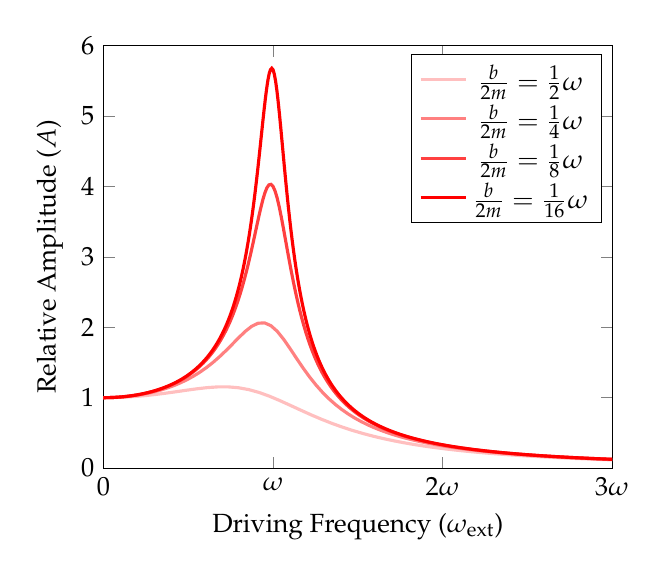
\begin{tikzpicture}[scale=.95]
      \begin{axis}[
          width=3.3in,
          xmin=0,xmax=3, xlabel=Driving Frequency ($\omega_\text{ext}$),
          xtick={0,1,2,3}, xticklabels={0,$\omega$,$2\omega$,$3\omega$},
          ymin=0,ymax=6, ylabel=Relative Amplitude ($A$),
          ytick={0,1,2,3,4,5,6}
        ]
        \addplot[
          color=red!25,
          samples=50,
          domain=0:3,
          very thick]{1/sqrt((1-x^2)^2+x^2)};
        \addlegendentry{$\frac b{2m}=\frac12\omega$}
        \addplot[
          color=red!50,
          samples=80,
          domain=0:3,
          very thick]{1/sqrt((1-x^2)^2+x^2/4)};
        \addlegendentry{$\frac b{2m}=\frac14\omega$}
        \addplot[
          color=red!75,
          samples=250,
          domain=0:3,
          very thick]{1/sqrt((1-x^2)^2+x^2/16)};
        \addlegendentry{$\frac b{2m}=\frac18\omega$}
        \addplot[
          color=red,
          samples=400,
          domain=0:3,
          very thick]{1/sqrt((1-x^2)^2+x^2/32)};
        \addlegendentry{$\frac b{2m}=\frac1{16}\omega$}
      \end{axis}
    \end{tikzpicture}

    \column{.5\textwidth}
    Plotting amplitude $A$ as a function of driving frequency
    $\omega_\text{ext}$ shows that:
    \begin{itemize}
    \item For a lightly damped system (i.e.\ small $b$), resonance response is
      highest when $\omega_\text{ext}\approx\omega\approx\omega_0$
    \item The smaller the damping constant $b$, the higher and narrower the
      peak is
    \end{itemize}
  \end{columns}
\end{frame}



\begin{frame}{Resonance}
  \eq{0in}{
    \boxed{\tan\phi=\frac{b\omega_a}{m(\omega_0^2-\omega_\text{ext}^2)}}
  }

  When $\omega_\text{ext}=\omega_0$ is substituted into the phase shift
  expression, the right-hand side becomes undefined. From this, we obtain a
  phase shift of $\phi=\pi/2$. Taking derivative of $x(t)$ for velocity $v(t)$,
  and substituting $\phi=\pi/2$:
  
  \eq{-.1in}{
    v(t)=\dot x
    =-A\omega_\text{ext}\sin(\omega_\text{ext}t-\frac{\pi}2)
    =A\omega_\text{ext}\cos(\omega_\text{ext}t)
  }
\end{frame}



\begin{frame}{Resonance}
  At resonance, the object is always moving in the same direction as the
  driving force:

  \vspace{-.3in}{\large
    \begin{align*}
      v(t)&=A\omega_\text{ext}\cos(\omega_\text{ext} t)\\
      F_a(t)&=F\cos(\omega_\text{ext} t)
    \end{align*}
  }

  This also makes sense from a work-energy perspective, because now the
  external force is doing positive work to the system.
\end{frame}



\begin{frame}{Resonance}
  \textbf{Resonance} is caused by in-phase excitation near the natural
  frequency. This means that:
  \begin{itemize}
  \item The frequency of the driving force is \emph{approximately} equal to the
    natural frequency of the damped oscillator:

    \eq{-.1in}{
      \omega_\text{ext}=\sqrt{\omega_0^2-\frac{b^2}{2m^2}}
      \quad\text{where}\quad\omega_0=\sqrt{\frac km}
    }

    For a lightly damped system, $\omega_\text{ext}\approx\omega\approx\omega_0$
  \item The driving force follows the motion of the oscillator.
  \end{itemize}
\end{frame}
\end{document}
